\section{Evaluation}
So far, we have presented a sound procedure and automated component-based framework for extracting the non-functional properties of generated code. In this section, we evaluate the implementation of our approach by explaining the design of our empirical study and the different methods we used to assess the effectiveness of our approach. 
The experimental material is available for replication purposes\footnote{\url{https://testingcodegenerators.wordpress.com/}}.
\subsection{Experimental Setup}
\subsubsection{Code Generators Under Test: HAXE compilers}
In order to test the applicability of our approach, we conduct experiments on a popular high-level programming language called HAXE and its code generators.

Haxe is an open source toolkit for cross-platform development which compiles to a number of different programming platforms, including JavaScript, Flash, PHP, C++, C\# and Java. Haxe involves many features: the Haxe language, multi-platform compilers, and different native libraries. 
The Haxe language is a high-level programming language which is strictly typed. This language supports both functional programming and object-oriented programming paradigms. It has a common type hierarchy, making certain API available on every targeted platform.
Moreover, Haxe comes with a set of compilers that translate manually-written code (in Haxe language) to different target languages and platforms. 
Haxe code can be compiled for applications running on desktop, mobile and web platforms. Compilers ensure the correctness of user code in terms of syntax and type safety.
Haxe comes also with a set of standard libraries that can be used on all supported targets and platform-specific libraries for each of them.

The process of code transformation and generation can be descibed as following: Haxe compilers analyzes the source code written in Haxe language then, the code is checked and parsed into a typed structure, resulting in a typed abstract syntax tree (AST). This AST is optimized and transformed afterwards to produce source code for target platform/language.

Haxe offers the option of choosing which platform to target for each program using a command-line tool. Moreover, some optimizations and debugging information can be enabled through CLI but in our experiments, we did not turned on any further options. 

\subsubsection{Cross-platform Benchmarking}
One way to prove the effectiveness of our approach is to create benchmarks. Thus, we use Haxe language, code generators, and a set of libraries to build a cross-platform benchmark based on this language. In fact, the provided benchmark is composed of a collection of cross-platform libraries that can be compiled to different targets\footnote{\url{http://thx-lib.org/}}. In these experiments, we are considering  five targets: Java, JS, C++, CS, and PHP. 
Each Haxe library comes with an API and a set of test suites. These tests, written in Haxe, represent a set of unit tests that covers the different features of the API. They can be executed within the target platform to test the functional behavior of generated programs. We use these test suites then, to generate a load and stress the target library. This can be useful to study the impact of this load on the resource usage of the system. In fact, we have removed all the tests that fail to compile to our five targets and we kept only test suites that are functionally correct. Thus, we run each test suite 1000 times to get comparable values in terms of resource usage.
Table 2 describes the Haxe libraries that we have selected from this benchmark to evaluate our
approach.

\begin{table}[h]
	\centering

	\begin{tabular}{|c|c|p{4.3cm}|}
		\hline
		\textbf{Library} & \textbf{\#TestSuites} & \textbf{Description} \\
		\hhline{|=|=|=|}
		Color  &  19 &  Color conversion from/to any color space   \\ \hline
		Core & 51  & Provides extensions to many types  \\ \hline
		Hxmath & 6  & A 2D/3D math library  \\ \hline
	    Format  &  4 & Format library such as dates, number formats   \\ \hline
		Promise & 3  & Library for lightweight promises and futures  \\ \hline
		Culture & 4  & Localization library for Haxe \\ \hline
		Math & 3  & Generation of random values \\ \hline
	\end{tabular}
		\caption{Description of selected benchmark libraries}
		\label{my-label}
\end{table}

\subsubsection{Evaluation Metrics Used}
We use to evaluate the efficiency of generated code using the following non-functional metrics:

-\textit{Memory Usage (MU)}:
It corresponds to the maximum memory consumption of the running container under test. Memory usage is measured in bytes.

-\textit{Execution Time (T)}:
Program execution time is measured in seconds.
 
\subsubsection{Setting up Infrastructure}
To assess our approach, we configure our previously proposed container-based infrastructure for non-functional testing of code generators in order to run experiments on the Haxe case study.
Figure 3 shows a big picture of the testing and monitoring infrastructure considered in these experiments.
\begin{table*}[h]
	\centering

	\resizebox{\linewidth}{!}{%
	\begin{tabular}{l|l|l|l|l|l|l|l|l|l|l|l|l|l|l|l|}
		\cline{2-16}
		& \multicolumn{3}{c|}{JAVA} & \multicolumn{3}{c|}{JS} & \multicolumn{3}{c|}{CPP} & \multicolumn{3}{c|}{CS} & \multicolumn{3}{c|}{PHP}                                                 \\ \cline{2-16} 
		& Avg    & Min    & Max     & Avg    & Min   & Max    & Avg    & Min    & Max    & Avg    & Min   & Max    & Avg                            & Min   & Max                             \\ \hline
		\multicolumn{1}{|l|}{Color}   & 2.72   & 0,69   & 28,58   & 1,67   & 0,52  & 16,66  & 3,52   & 0,37   & 48,31  & 3,81   & 0,52  & 45,97  & \cellcolor[HTML]{C0C0C0}23,16  & 0,61  & \cellcolor[HTML]{C0C0C0}279,27  \\ \hline
		\multicolumn{1}{|l|}{Core}    & 0,82   & 0,57   & 8,71    & 0,86   & 0,51  & 14,01  & 0,61   & 0,42   & 8,11   & 0,98   & 0,50  & 21,60  & \cellcolor[HTML]{C0C0C0}49,52  & 0,47  & \cellcolor[HTML]{C0C0C0}2479,07 \\ \hline
		\multicolumn{1}{|l|}{Hxmath}  & 1,62   & 0,66   & 3,38    & 1,1    & 0,54  & 2,04   & 0,81   & 0,39   & 1,42   & 1,64   & 0,56  & 4,01   & \cellcolor[HTML]{C0C0C0}26,53  & 1,06  & \cellcolor[HTML]{C0C0C0}73,44   \\ \hline
		\multicolumn{1}{|l|}{Format}  & 2,19   & 0,71   & 5,03    & 2,23   & 0,60  & 5,402  & 2,57   & 0,37   & 7,67   & 4,97   & 0,54  & 12,38  & \cellcolor[HTML]{C0C0C0}93,53  & 1,11  & \cellcolor[HTML]{C0C0C0}220,75  \\ \hline
		\multicolumn{1}{|l|}{Promise} & 0,89   & 0,63   & 1,72    & 1,44   & 0,54  & 2,09   & 0,69   & 0,39   & 1,12   & 0,99   & 0,48  & 1,71   & \cellcolor[HTML]{C0C0C0}11,96  & 1,13  & \cellcolor[HTML]{C0C0C0}31,18   \\ \hline
		\multicolumn{1}{|l|}{Culture} & 0,64   & 0,55   & 0,82    & 0,50   & 0,46  & 0,57   & 0,44   & 0,37   & 0,62   & 0,50   & 0,43  & 0,65   & 1,46                           & 0,61  & 3,79                            \\ \hline
		\multicolumn{1}{|l|}{Math}    & 5,26   & 0,98   & 12,51   & 1,66   & 0,75  & 3.10   & 6,30   & 0,93   & 16,29  & 5,75   & 0,94  & 14,14  & \cellcolor[HTML]{C0C0C0}523,17 & 55,45 & \cellcolor[HTML]{C0C0C0}1448,9  \\ \hline
	\end{tabular}%
}
	\caption{Execution time stats}
	\label{my-label}
\end{table*}
% Please add the following required packages to your document preamble:
% \usepackage[table,xcdraw]{xcolor}
% If you use beamer only pass "xcolor=table" option, i.e. \documentclass[xcolor=table]{beamer}


\begin{table*}[h]
	\centering
	
	\resizebox{\linewidth}{!}{%
\begin{tabular}{l|l|l|l|l|l|l|l|l|l|l|l|l|l|l|l|}
	\cline{2-16}
	& \multicolumn{3}{c|}{JAVA} & \multicolumn{3}{c|}{JS} & \multicolumn{3}{c|}{CPP} & \multicolumn{3}{c|}{CS} & \multicolumn{3}{c|}{PHP}   \\ \cline{2-16} 
	& Avg     & Min   & Max     & Avg     & Min  & Max    & Avg     & Min  & Max     & Avg     & Min  & Max    & Avg     & Min    & Max     \\ \hline
	\multicolumn{1}{|l|}{Color}   & 115,98  & 0,53  & 1362,55 & 62,33   & 0,70 & 900,70 & 169,90  & 0,16 & 2275,49 & 87,51   & 0,42 & 1283,3 & 173,69  & 0,81   & 2189,85 \\ \hline
	\multicolumn{1}{|l|}{Core}    & 21,94   & 0,52  & 1057,32 & 2,19    & 0,64 & 59,96  & 1,89    & 0,29 & 35,97   & 2,38    & 0,59 & 42,92  & 2,49    & 0,46   & 32,91   \\ \hline
	\multicolumn{1}{|l|}{Hxmath}  & 121,47  & 0,70  & 389,72  & 37,23   & 1,37 & 111,68 & 96,15   & 1,20 & 296,43  & 50,19   & 0,81 & 156,40 & 472,26  & 1,11   & 1192,98 \\ \hline
	\multicolumn{1}{|l|}{Format}  & 214,04  & 0,67  & 685,90  & 38,93   & 2,42 & 92,34  & 70,29   & 1,12 & 204,85  & 31,11   & 1,08 & 69,16  & 177,17  & 0,58   & 385,11  \\ \hline
	\multicolumn{1}{|l|}{Promise} & 32,85   & 1,23  & 128,29  & 31,65   & 0,54 & 55,29  & 0,93    & 0,45 & 1,73    & 12,85   & 0,87 & 34,49  & 57,96   & 0,65   & 134,20  \\ \hline
	\multicolumn{1}{|l|}{Culture} & 2,20    & 1,15  & 4,04    & 1,12    & 0,70 & 1,59   & 1,68    & 1,35 & 2,02    & 3,34    & 0,55 & 11,20  & 10,11   & 1,11   & 36,32   \\ \hline
	\multicolumn{1}{|l|}{Math}    & 353,18  & 1,21  & 831,44  & 165,71  & 0,93 & 493,66 & 597,02  & 1,61 & 1492,97 & 312,37  & 3,37 & 806,33 & 1448,45 & 626,83 & 3088,15 \\ \hline
\end{tabular}%
}
\caption{Memory stats}
\label{my-label}
\end{table*}
First, we create a new Docker image in where we install the Haxe code generators and compilers (through the configuration file "Dockerfile"). Then a new instance of that image is created. It takes as an input the Haxe library we would to test and the list of test suites (step 1). It produces as an output the source code and binaries that have to be executed. These files are saved in a shared repository.
In Docker environment, this repository is called Data Volume. A data volume is a specially-designated directory within containers that share data with the host machine. So, when
we execute the generated test suites, we provide a shared volume with
the host machine so that, binaries can be executed in the execution container (Step 2). In fact, for the code execution we created, as well, a new Docker image in where we install all execution tools and environments such as php interpreter, NodeJS, etc. 

In the meantime, while running test suites inside the container, we collect runtime resource usage data using cAdvisor (step 3). The cAdvisor Docker image does not need any configuration on the host machine. We have just to run it on our host machine. It will then have access to resource usage and performance characteristics of all running containers. This image uses the cgroups mechanism described previously to collect, aggregate, process, and export ephemeral real-time information about running containers. Then, it reports all statistics via web UI (\textit{http://localhost:8080}) to view live resource consumption of each container. cAdvisor has been widely used in different projects such as Heapster\footnote{\url{https://github.com/kubernetes/heapster}} and Google Cloud Platform\footnote{\url{https://cloud.google.com/}}. In this experiment, we choose to gather information about the memory usage of running container.
Afterwards, we record these data into a new time-series database using our InfluxDB back-end container (step 4). Thus, we define its corresponding ip port into the monitoring component so that, container statistics are sent over TCP port (e.g., \textit{8083}) exposed by the database component. 

Next, we run Grafana and we link it to InfluxDB by setting up the data source port 8086 so that, it can easily request data from the database. We recall that InfluxDB also provides a web UI to query the database and show graphs (step 5). But, Grafana let us display live results over time in much pretty looking graphs. Same as InfluxDB, we use SQL queries to extract non-functional metrics from the database for visualization and analysis (step 6). In our experiment, we are gathering the maximum memory usage values without presenting the graphs of resource usage profiles.
 
 

\begin{figure}[hbt]
	\centering
	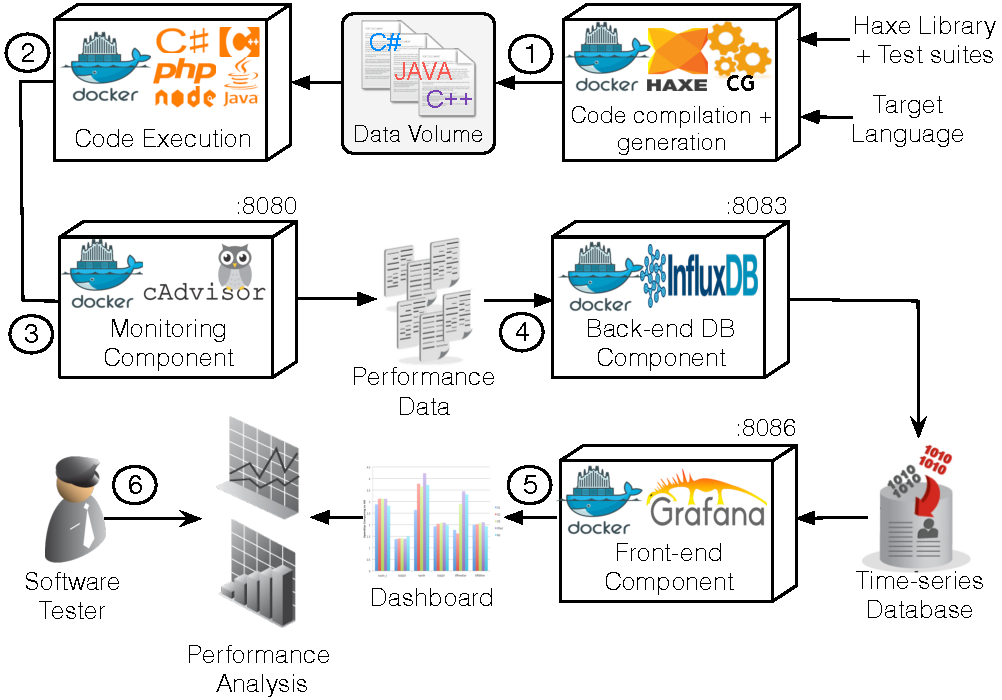
\includegraphics[width=1\linewidth]{Ressources/settingup.pdf}
	\caption{Comparison of average memory consumption and execution time of FFmpeg containers compiled with standard GCC optimization options}
\end{figure}
To obtain comparable and reproducible results, we use the
same hardware across all experiments: an AMD A10-7700K
APU Radeon(TM) R7 Graphics processor with 4 CPU cores
(2.0 GHz), running Linux with a 64 bit kernel and 16 GB of
system memory.

\subsection{Experimental Results}
The experimental consisted of comparing the execution time and memory consumption on the following targets: Java, JS, C++, CS, and PHP.

% Please add the following required packages to your document preamble:
% \usepackage[table,xcdraw]{xcolor}
% If you use beamer only pass "xcolor=table" option, i.e. \documentclass[xcolor=table]{beamer}

\subsection{Discussions}
\iffalse
In this section, we evaluate the implementation of our approach across two case studies. These experiments aim at answering the following research questions:

\textbf{RQ1:} How do standard GCC optimization levels influence on the resource consumption of generated programs?
To answer this question, we apply standard optimization options to FFmpeg library. Then, we evaluate the memory footprint and execution time of running FFmpeg command lines and we compare the results. The goal of this initial experiment is to
provide an understanding of the performance of generated code by GCC.

\textbf{RQ2:} To what extent can the proposed diversity-based exploration of optimization options impact the resource consumption of generated programs?
In a second experiment, we assess our NS approach for automatic optimization sequences generation by comparing the results found when applying standard optimization sequences to new results provided by our approach. The experimental results show that our novelty-based approach can produce optimization sequences with good performance and less resource consumption
than standard optimization levels in GCC. In this experiment, we study the correlation between execution time and memory consumption of generated code.

These two case studies  also enable to validate the global approach for non functional testing of code generators using system containers. 



\subsection{Case Study 1: FFmpeg}
In the first experiment, we set up our infrastructure for testing and monitoring of generated code. In this part, we compile the FFmpeg library using standard GCC optimizations(O1, O2, O3, Ofast) and we study the impact of these optimizations on memory consumption and execution time using our Docker-based infrastructure.

\subsubsection{FFmpeg: Multimedia Encoding Library}
FFmpeg\footnote{\url{https://www.ffmpeg.org/}} is a complete, cross-platform solution to record, convert, and stream audio and video. It is a very fast video and audio converter. It includes libraries of audio/video codecs and a command-line program for transcoding multimedia files. FFmpeg allows different types of multimedia conversion and that depends on the input and output format (video, audio, subtitle, attachment, data). Video/audio processing with FFmpeg usually need high-performance requirements and an important amount of resources in term of memory usage. So, testing GCC on top of this library is very interesting in order to compare resource usage profiles. 
\subsubsection{Docker-based Infrastructure for Monitoring FFmpeg Containers}


The goal of this experiment is to compile FFmpeg with standard GCC optimization options and run FFmpeg command examples on top of different versions in order to compare the memory usage profiles and execution time of different variants using our test architecture. An overview of the different components involved in testing and monitoring of FFmpeg containers is shown in Figure 2. 
First, we compile FFmpeg library with different optimization options  (O0, O1, O2, O3 and Ofast) in order to produce 5 variants of FFmpeg. This is done within Docker containers. We configure each container to install FFmpeg with a specific configuration and we upload all FFmpeg images in Docker Hub\footnote{https://hub.docker.com/}.
Docker Hub is a cloud-based registry service for building and shipping application or service containers. We use it for building, saving, and managing all our Docker images.

Afterwards, we execute the same stressload (FFmpeg examples) within each FFmpeg instance container. We choose 15 FFmpeg command examples that cover multiple domains\footnote{http://goo.gl/11VLYM} like video conversion, sound extraction, encoding file for iPod or PSP, etc. This list of examples is saved in a script file that should be executed later within FFmpeg containers. The media files needed for encoding are saved in a shared repository. In Docker environment, we call this repository the “Data Volume”. A data volume is a specially-designated directory within containers that share data with the host machine. Data is persistent and independent of container's life cycle. So, when we run FFmpeg containers we provide a shared volume with the host machine (where the media files are located). As well, the list of FFmpeg commands to execute is mounted in this volume so that, we can execute the same workload each time we run a new container.
Before running FFmepg workload on different containers, we run monitoring components (cAdvisor, InfluxDB and Grafana) to start gathering usage statistics.
In fact, in this experiment, we choose to gather statistics about memory consumption and execution time of different containers. 

To obtain comparable and reproducible results, we use the same hardware across all experiments: an AMD A10-7700K APU Radeon(TM) R7 Graphics processor with 4 CPU cores (2.0 GHz), running Linux with a 64 bit kernel and 16 GB of system memory.

\subsubsection{Experimental Results}
\begin{figure}[!t]
	\centering
	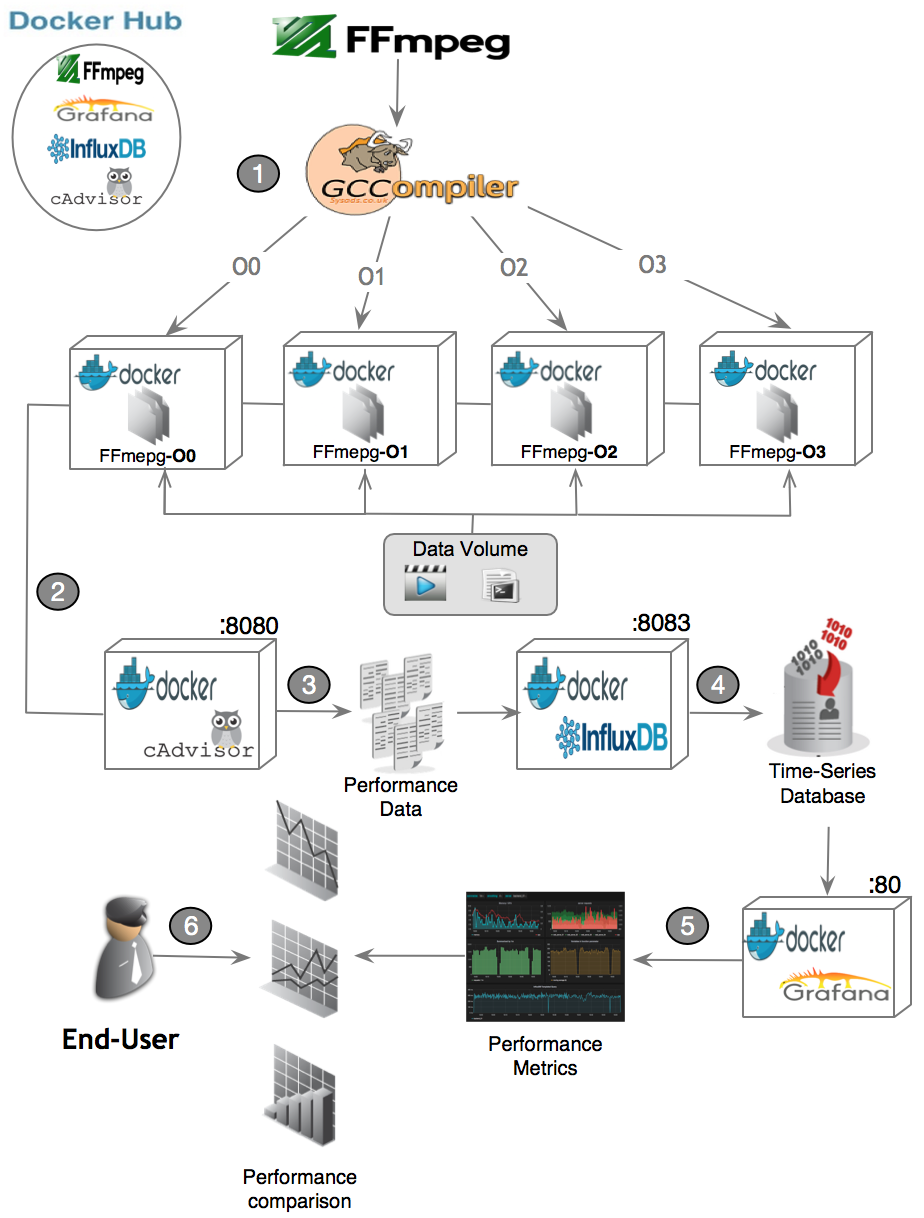
\includegraphics[width=1.\linewidth]{Ressources/infra_ffmpeg.png}
	\caption{Overview of the different components involved in testing and monitoring of FFmpeg containers}
\end{figure}


\begin{figure}[tbh]
	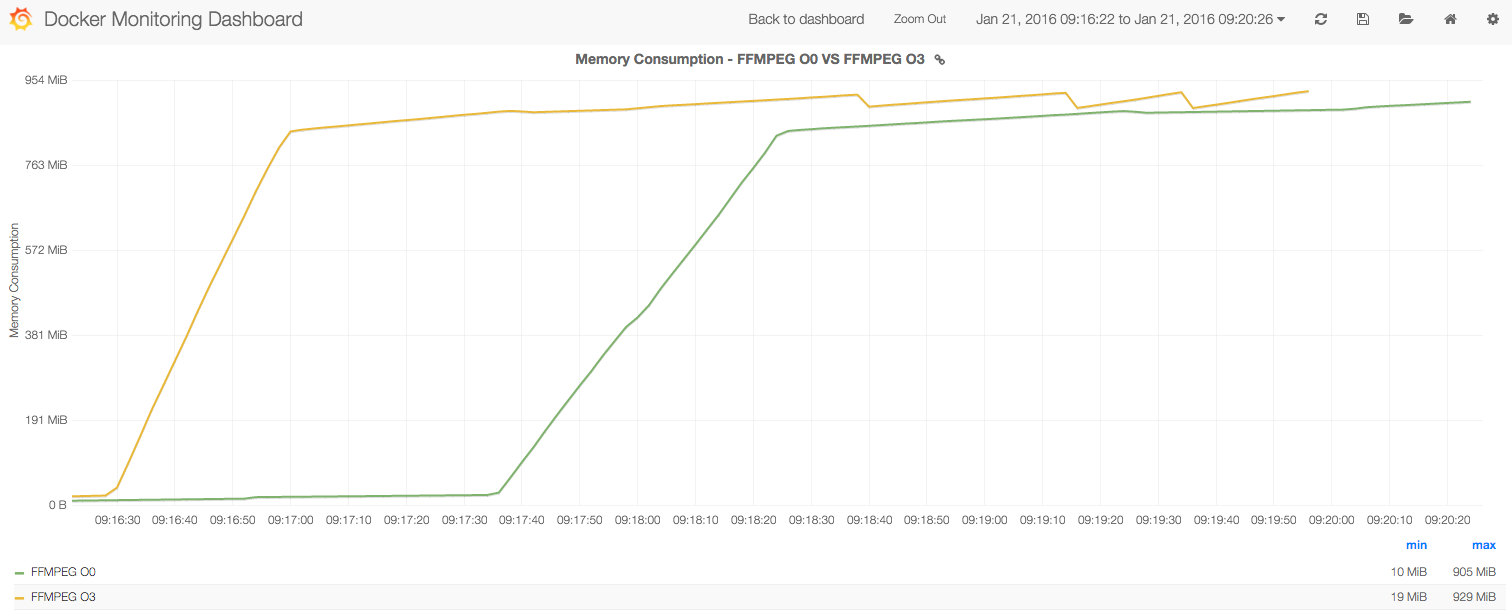
\includegraphics[width=1\linewidth]{Ressources/infra_stats.png}
	\caption{Snapshot of runtime memory consumption profiles of FFmpeg containers compiled with O0 (no optimization) and O3 options}
	%		\label{AAA}
\end{figure}

In this first part of experiments with FFmpeg, we compare a zero-level optimization container (FFmpeg-O0) with a high-level optimization one (FFmpeg-O3) in order to study the impact of optimizations on memory usage and execution time. Figure 3 shows runtime statistics of running two FFmpeg containers O0 and O3 with the same input workload. This chart depicts a snapshot of our visualization component web UI. It presents the memory usage profiles of two components (FFmpeg O0 and O3) started in the same time and running in parallel. Visually, we can see that the execution time of O3 (yellow) is faster than O0 (green) since O3 execution ended before O0. However, we can see that memory usage remains higher than O0 from the beginning to the end of running FFmpeg examples. 

To better understand the resource usage of optimized code, we run the same experiment for all FFmpeg containers and we collect the same metrics. Figure 4 presents a comparison of average memory usage and execution time of FFmpeg containers compiled with all standard GCC optimization options. We notice that the memory usage increases as soon as we apply more aggressive optimization. However, when we apply higher optimization level, we clearly improve the execution time compared to O0. For example, O3 and Ofast have the highest memory consumption (100 MBytes more than O0) and best execution time (speedup around 1.8) which can be inconvenient for systems with limited resources.

This results explain that optimizing for execution time (for the case of FFmpeg) is not always efficient regarding memory usage and unfortunately, optimizations may influence negatively the system resources.
\begin{figure}[hbt]
	\centering
	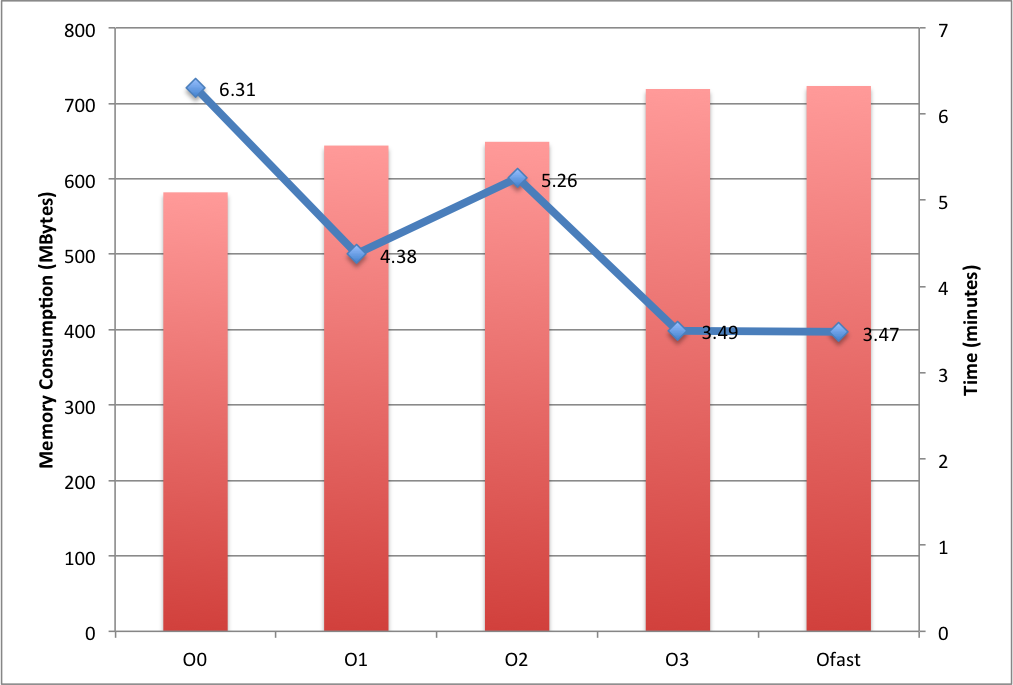
\includegraphics[width=1\linewidth]{Ressources/infra_ffmpeg_plot1.png}
	\caption{Comparison of average memory consumption and execution time of FFmpeg containers compiled with standard GCC optimization options}
\end{figure}


\subsection{Case Study 2: Novelty-based Exploration of Optimization Sequences}
In this second case study, we assess the performance of GCC compiler across different benchmark programs. The goal of this experiment is to show that our approach for exploring the search space of optimizations is able to generate efficient code that yields to less resource consumption than GCC default optimizations.
\subsubsection{Setting Up Infrastructure}
\begin{figure}[b]
	\centering
	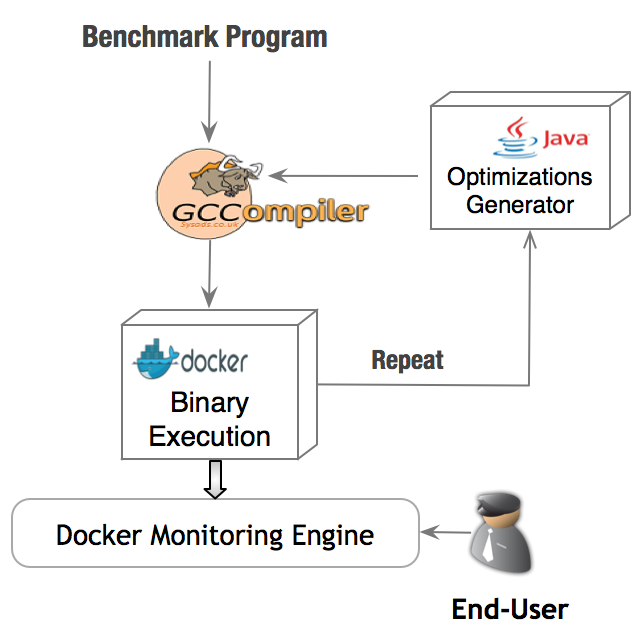
\includegraphics[scale=0.50]{Ressources/infra_novelty.png}
	\caption{Overall process of monitoring code generated by GCC}
	
%	\vspace*{-5cm}
	
\end{figure}
For this experiment, we keep the same architecture settings as first case study. However, we provide a more generalized approach for automatic testing of code generators using system containers. So, starting from a list of optimizations defined by the user, an input program and a specific target compiler, we are able to execute and monitor optimized code. Figure 5 shows more details about this process. First, our novelty-based test sequences generator generates a huge amount of diverse optimizations. We compile an input program with these generated sequences using GCC. Then, we execute produced binaries sequentially within isolated Docker containers (Docker image with GCC version 4.8.4 installed above). We keep the same monitoring chain to gather resource usage of running containers. This process is repeated until the end of generated sequences. Finally, end-users (testers) can access to resource consumption statistics through InfluxDB or Grafana Web UI to compare the impact of optimizations on resource consumption. In this example too, we choose to focus on studying the trade-off memory usage/execution time. 
\subsubsection{Benchmark programs}
To explore the impact of compiler optimizations a set of input programs are needed. We run experiments on commonly used benchmarks named Collective Benchmark (cBench)~\cite{fursin2009collective}. It is a collection of open-source sequential programs in C targeting specific areas of the embedded market. It comes with multiple datasets assembled by the community to enable realistic benchmarking and research on program and architecture optimization. cBench contains more than 20 C programs. The following table describes programs that we have selected from this benchmark to evaluate our approach.
\begin{table}[h]
	\begin{center}
		\begin{tabular}{|c|c|p{3.9cm}|}
			\hline
			\textbf{Program} & \textbf{Source lines} & \textbf{Description}\\
			\hline
			automative\_susan\_s & 1376 & Image recognition package\\
			\hline
			bzip2e & 5125 & Compress any file
			source code \\
			\hline
			bzip2d & 5125 & Decompress zipped files \\
			\hline
			office\_rsynth & 4111 & Text to speech program produced by integrating various pieces of code\\
			\hline
			consumer\_tiffmedian& 15870 & Apply the median cut algorithm to data in a TIFF file
			\\
			
			\hline
			 consumer\_tiffdither& 15399 & Convert a greyscale image to bilevel using dithering
			 \\
			\hline
			
		\end{tabular}
		
	\end{center}
	\caption {Description of selected benchmark programs}
\end{table}
\subsubsection{Novelty Parameters}
%Our experiments use the classical NS algorithm, where we evolve a set of optimization sequences through generations.
NS is implemented as described in Section 3.
The first step in the process of selection is to evaluate each individual and compute its novelty score. Novelty is calculated for each organism by taking the mean of its 15 lowest dissimilar optimization sequences (considering all sequences in the current population and in the archive). 
Then, to create next populations, an elite of the 10 most novel organisms is copied unchanged, after which the rest of the new population is created by tournament selection according to novelty. Standard genetic programming crossover and mutation operators are applied to these novel sequences in order to produce offspring individuals and fulfill the next population.
In the meanwhile, individuals that get a score higher than the threshold T they are automatically added to the archive as well. 
In fact, this threshold is dynamic. Every 150 evaluations, we check how many individuals have been copied into the archive. If this number is below 3, the threshold is increased by multiplying it by 0.95, whereas if solutions added to archive are above 3, the threshold is decreased by multiplying it by 1.05. 
Moreover, as the size of the archive grows, the nearest-neighbor calculations that determine the novelty scores for individuals become more computationally demanding. So to avoid having low accuracy of novelty, we choose to bound the size of the archive. Hence, it follows a first-in first-out data structure which means that when a new solution gets added, the oldest solution in the novelty archive will be discarded. Thus, we ensure individuals diversity by removing old sequences that may no longer be reachable from the current population.

The parameters of the algorithm were tuned individually in preliminary experiments. For each parameter, a set of values was tested. The parameter values chosen are the mostly used in the literature~\cite{lehman2008exploiting}. The value that yielded the highest performance scores was chosen. The resulting parameter values are listed in Table 4.
\begin{table}
		\caption{Parameters of NS algorithm}
		\begin{tabular}{ l l || l l }
			Parameter & Value & Parameter & Value \\	\hline
			Novelty nearest-k  & 15 &  Tournament size & 2\\ 
			Add archive prob. & 30 &  Mutation prob. & 0.1\\  
			Max archive size & 500 &  Crossover & 0.5  \\  
			Population size & 100 &  Nb generations &  100 \\  
			Individual length & 76 & Elitism & 10  \\ 
			Scaling archive prob. & 0.05 & Solutions added to archive & 3  \\ 
		\end{tabular}
\end{table}

\subsubsection{Experimental results}

The goal of this experiment is to compare novelty-based generated sequences to standard GCC optimizations in term of memory consumption. Figure 6 shows this comparison across different benchmark programs. It presents the percentage of saved memory of standard and novelty optimizations over O0 level (no optimization applied).
 
\begin{figure}[!ht]
	\centering
	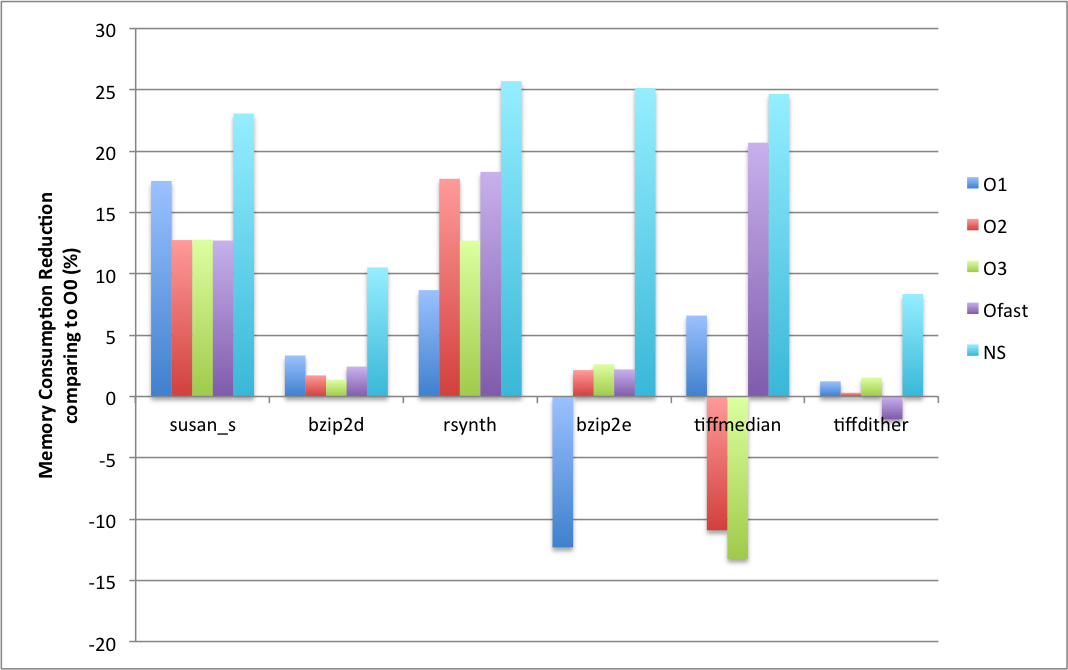
\includegraphics[width=1.\linewidth]{Ressources/infra_novelty_stat3.png}
	\caption{Evaluating the amount of saved memory after applying standard optimization options compared to best generated optimization using NS}
\end{figure}

For NS, we select the best sequence that reduces the memory consumption and we compare it to the memory footprint of O0, O1, O2, O3 and Ofast versions. The results show clearly that NS outperforms standard optimizations for all benchmark programs. Using NS, we are able to reach a maximum memory consumption reduction of almost 26\% for the case rsynth program against a maximum of 18\% reduction using Ofast option. We remark as well that the impact of applying standard optimizations on memory consumption for each program differs from one program to another. Using O1 for bzip2e and O2, O3 for tiffmedian can even increase the memory consumption by almost 13 \% (like the FFmpeg experiments). This agrees to the idea that standard optimizations does not produce always the same impact results on resource consumption and may be highly dependent on the benchmark and the source code they have been tested on. Our approach can clearly provide an alternative to catch most relevant optimization sequence regarding resource consumptions.

To study the correlation between execution time and memory consumption of running programs, we present in Figure 7 an evaluation of the speedup. We compare the speedup (according to O0) of the best optimization sequences by NS (gathered in Figure 6) with standard optimization options. 
The first observation is that optimizations yield to high level of speedup for all benchmark programs (between 1.5 and 4.3).
The second observation we can make is that different optimizations do not differ too much in term of execution time. We  distinguish that Ofast is slightly more efficient for all programs and NS sequence has almost the same speedup as Ofast. 
The results of this experiments shows that optimizing for memory usage using NS does not affect programs execution time and we demonstrate that we can find optimizations that reduce memory usage while guaranteeing program performance.
\begin{figure}[!ht]
	\centering
	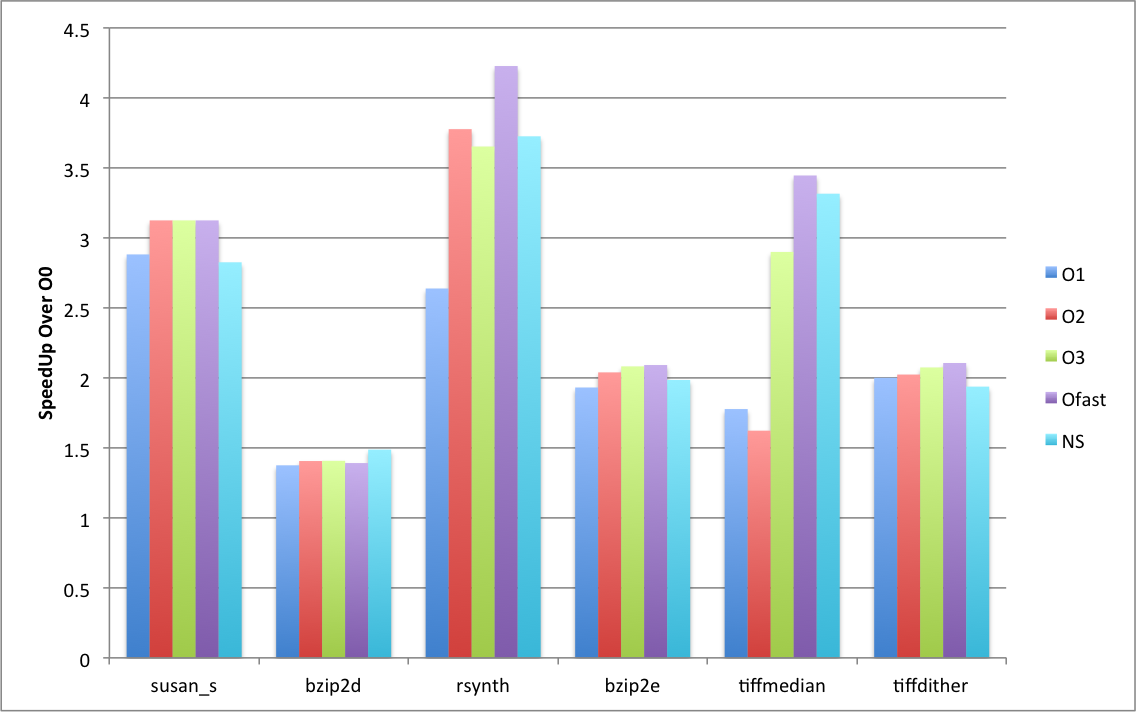
\includegraphics[width=1.\linewidth]{Ressources/infra_novelty_stat2.png}
	\caption{Evaluating the speedup after applying standard optimization options compared to best generated optimization using NS}
\end{figure}

\fi